% Euclidean Handout Number Twelve
\documentclass{tufte-handout}

%\geometry{showframe}% for debugging purposes -- displays the margins

%%%% Packages to make things pretty
\usepackage{amsmath,amsthm}
\usepackage{booktabs}
\usepackage{graphicx}
\setkeys{Gin}{width=\linewidth,totalheight=\textheight,keepaspectratio}
\graphicspath{{graphics/}}
\usepackage{units}
\usepackage{fancyvrb}
\fvset{fontsize=\normalsize}
\usepackage{multicol}
\usepackage{pdfpages}

%%%% Theorem Environments
\theoremstyle{definition}
\swapnumbers
\newtheorem{problem}{Problem}[section]
\newtheorem{conjecture}[problem]{Conjecture}
\newtheorem*{definition}{Definition}
\newtheorem*{theorem}{Theorem}
\newtheorem{question}[problem]{Question}
\newtheorem{challenge}[problem]{Challenge}
\newtheorem*{postulate}{Postulate}

%%%%%

\title{Euclidean Geometry:\\An Introduction to Mathematical Work}
\author[]{Math 3600}
\date{Fall 2020}

\begin{document}

\maketitle

\begin{marginfigure}
    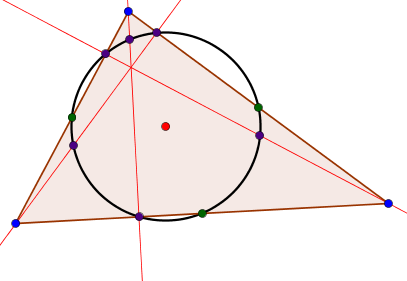
\includegraphics{NPC}
\end{marginfigure}

\setcounter{section}{12}
\section{More Advanced Constructions}

\begin{definition}\label{defn:circumscribed}
A circle is said to be \emph{circumscribed} about a figure if the figure lies in the interior of the circle, except for the vertices which lie on the circle.

A circle is said to be \emph{inscribed} in a figure if the circle lies in the interior of the figure and is tangent to each of the sides of the figure.
\end{definition}

\begin{challenge}\label{chal:triangle-inscribe-circle}
Construct a circle inscribed in a given triangle $ABC$. (par 13)
\end{challenge}

\begin{challenge}\label{chal:triangle-circumscribe-circle}
Construct a circle circumscribed about a given triangle $ABC$. (par 7)
\end{challenge}



\begin{challenge}\label{chal:cut-segment-by-circle}
Given a line $\ell$, a line segment $d$ and a point $O$, construct a circle with center $O$ that cuts off a segment from line $\ell$ which is congruent to $d$.
\end{challenge}



\begin{challenge}\label{chal:three-perp-circles}
Construct three circles such that each pair meets at right angles. (par 10)
\end{challenge}

\begin{challenge}\label{chal:cut-circle-by-segment}
Given a segment $d$, a circle with center $O$ and a point $P$ inside the circle, construct a line through $P$ on which the circle cuts off a segment congruent to $d$.

When exactly is this construction possible?
\end{challenge}


\begin{challenge}\label{chal:triangle-problem}
Given a segment $AB$ and an angle $\alpha$ and given another segment $d$, construct a triangle $ABC$ with base equal to $AB$, angle $\alpha$ at $C$ and such that $AC + CB = d$.

Exactly how often is this construction possible? How many ways can the conditions be met?
\end{challenge}


\begin{challenge}\label{chal:double-tangent}
Given two circles $\Gamma$ and $\Gamma'$ with centers $O, O'$, respectively, construct a line tangent to both circles.

How many such lines are there?
\end{challenge}


\vfill
\end{document}

%sagemathcloud={"zoom_width":100}